\documentclass[11pt]{article}

\usepackage[a4paper]{geometry}
\geometry{left=2.0cm,right=2.0cm,top=2.5cm,bottom=2.5cm}

\usepackage{ctex} % 支持中文的LaTeX宏包
\usepackage{amsmath,amsfonts,graphicx,subfigure,amssymb,bm,amsthm,mathrsfs,mathtools,breqn} % 数学公式和符号的宏包集合
\usepackage{algorithm,algorithmicx} % 算法和伪代码的宏包
\usepackage[noend]{algpseudocode} % 算法和伪代码的宏包
\usepackage{fancyhdr} % 自定义页眉页脚的宏包
\usepackage[framemethod=TikZ]{mdframed} % 创建带边框的框架的宏包
\usepackage{fontspec} % 字体设置的宏包
\usepackage{adjustbox} % 调整盒子大小的宏包
\usepackage{fontsize} % 设置字体大小的宏包
\usepackage{tikz} % 绘制图形和使用颜色的宏包
\usepackage{pgfplots} % 绘制数据图表的宏包
\pgfplotsset{compat=1.17} % 设置pgfplots版本兼容性
\usetikzlibrary{arrows.meta,positioning} % TikZ箭头库和定位库
\usepackage{float} % 支持[H]浮动体位置参数
\usepackage{multicol} % 多栏排版的宏包
\usepackage{multirow} % 表格中合并单元格的宏包
\usepackage{pdfpages} % 插入PDF文件的宏包
\RequirePackage{listings} % 在文档中插入源代码的宏包
\usepackage{wrapfig} % 文字绕排图片的宏包
\usepackage{bigstrut,multirow,rotating} % 支持在表格中使用特殊命令的宏包
\usepackage{booktabs} % 创建美观的表格的宏包
\usepackage{threeparttable} % 支持表格注释的宏包
\usepackage{circuitikz} % 绘制电路图的宏包
\usepackage{hyperref} % 创建超链接的宏包
\usepackage[inline]{enumitem} % 自定义列表格式的宏包，支持行内列表

\definecolor{dkgreen}{rgb}{0,0.6,0}
\definecolor{gray}{rgb}{0.5,0.5,0.5}
\definecolor{mauve}{rgb}{0.58,0,0.82}
\lstset{
  frame=tb,
  aboveskip=3mm,
  belowskip=3mm,
  showstringspaces=false,
  columns=flexible,
  framerule=1pt,
  rulecolor=\color{gray!35},
  backgroundcolor=\color{gray!5},
  basicstyle={\small\ttfamily},
  numbers=none,
  numberstyle=\tiny\color{gray},
  keywordstyle=\color{blue},
  commentstyle=\color{dkgreen},
  stringstyle=\color{mauve},
  breaklines=true,
  breakatwhitespace=true,
  tabsize=3,
}


\usepackage[capitalize]{cleveref}
\Crefname{section}{Section}{Sections}
\Crefname{table}{Table}{Tables}
\crefname{table}{Table.}{Tabs.}

\setmainfont{Palatino Linotype}
\setCJKmainfont{SimSun}[BoldFont=SimHei, ItalicFont=KaiTi]
\setCJKsansfont{SimHei}
\setCJKmonofont{FangSong}
\punctstyle{kaiming}
% 偏好的几个字体, 可以根据需要自行加入字体ttf文件并调用
\renewcommand{\emph}[1]{\textit{#1}}

%改这里可以修改实验报告表头的信息
\newcommand{\experiName}{密里根油滴实验和粘滞系数实验}
\newcommand{\supervisor}{张凯轩}
\newcommand{\name}{邓思豪}
\newcommand{\studentNum}{2023K8009909008}
\newcommand{\class}{3}
\newcommand{\group}{01}
\newcommand{\seat}{5}
\newcommand{\dateYear}{2025}
\newcommand{\dateMonth}{12}
\newcommand{\dateDay}{15}
\newcommand{\room}{西实206}
\newcommand{\others}{$\square$}


\begin{document}



\begin{center}
    \LARGE \bf 《\, 基\, 础\, 物\, 理\, 实\, 验\, 》\, 实\, 验\, 报\, 告
\end{center}

\begin{center}
    \noindent \emph{实验名称}\underline{\makebox[25em][c]{\experiName}}
    \emph{指导教师}\underline{\makebox[8em][c]{\supervisor}}\\
    \emph{姓名}\underline{\makebox[6em][c]{\name}} 
    % 如果名字比较长, 可以修改box的长度"6em"
    \emph{学号}\underline{\makebox[10em][c]{\studentNum}}
    \emph{分班分组及座号} \underline{\makebox[5em][c]{\class \ -\ \group \ -\ \seat }\emph{号}} （\emph{例}:\, 1\,-\,04\,-\,5\emph{号}）\\
    \emph{实验日期} \underline{\makebox[3em][c]{\dateYear}}\emph{年}
    \underline{\makebox[2em][c]{\dateMonth}}\emph{月}
    \underline{\makebox[2em][c]{\dateDay}}\emph{日}
    \emph{实验地点}\underline{\makebox[6em][c]{\room}}
    \emph{调课/补课} \underline{\rule{1.5ex}{1.5ex}是}
    \emph{成绩评定} \underline{\hspace{5em}}
    {\noindent}
    \rule[8pt]{17cm}{0.2em}
\end{center}

\section{实验目的}

\begin{enumerate}
    \item 通过学习密立根油滴实验的巧妙设计，体会一种微观量的宏观测量方法。
    \item 验证电荷的不连续性以及测量基本电荷电量。
    \item 通过对实验仪器的调整、油滴的选择、耐心地跟踪和测量以及数据的处理等，培养学生严肃认真和一丝不苟的科学实验方法和态度。
    \item 了解 CCD 光学成像系统的工作原理。
\end{enumerate}

\section{实验仪器}
\subsection{油滴实验实验仪器}

DH0605 型密立根油滴仪，由主机，CCD 成像系统，油滴盒，监视器等组成。

% --- 图 4 区域 ---
\begin{figure}[htbp]
    \centering
    % 左侧放置图片（请替换为您保存的图片文件名）
    \begin{minipage}[c]{0.5\textwidth}
        \centering
        
\includegraphics[width=\textwidth]{figure4.png} 
    \end{minipage}
    \hfill
    % 右侧放置编号说明
    \begin{minipage}[c]{0.45\textwidth}
        \small
        \begin{tabular}{lll}
            1. 喷雾室 & 2. 喷雾口 & 3. 进油控制开关 \\
            4. 进油孔 & 5. 上极板 & 6. 观察孔 \\
            7. 下极板 & 8. 落油孔 & 9. 油滴室
        \end{tabular}
    \end{minipage}
    \vspace{0.5em}
    \caption{\textbf{油滴盒示意图}}
\end{figure}

% --- 图 5 区域 ---
\begin{figure}[htbp]
    \centering
    % 放置主仪器图片
    
\includegraphics[width=0.9\textwidth]{figure5.png}
    
    \vspace{1em}
    % 下方的详细编号列表
    \small
    \begin{tabular}{p{4.5cm} p{2.5cm} p{2.5cm} p{2.5cm}}
        1. 视频输出接口，与监视器相连 & 2. CCD 相机 & 3. 调焦旋钮 & 4. 光学系统 \\
        5. 物镜镜头 & 6. 观察孔 & 7. LED 光源 & 8. 水平调节螺钉 \\
    \end{tabular}
    
    \begin{tabular}{p{2.5cm} p{3.5cm} p{2cm} p{2cm} p{2cm}}
        9. 电压调节旋钮 & 10. 开始键 & 11. 0V 键（极板不加电） & 12. 平衡键 & 13. 确认键 \\
        14. 结束键 & 15. 工作键 & 16. 提升键 & 17. 重做键 & \\
    \end{tabular}
    
    \vspace{0.5em}
    \caption{\textbf{DH0605 密立根油滴仪示意图}}
\end{figure}

\subsection{粘滞系数实验仪器}

\subsubsection{WT-CNZ 粘滞系数测量仪}

\begin{figure}[htbp]
    \centering
    % 图1和图2并排显示
    \begin{minipage}[b]{0.45\textwidth}
        \centering
        
\includegraphics[width=\textwidth]{fig1.png} % 请替换为您的图片文件名
        \caption{WT-CNZ 粘滞系数测量仪}
    \end{minipage}
    \hfill
    \begin{minipage}[b]{0.45\textwidth}
        \centering
        
\includegraphics[width=0.8\textwidth]{fig2.png} % 请替换为您的图片文件名
        \caption{水平调节装置}
    \end{minipage}
\end{figure}

变温粘度仪的外型如图 1 所示。待测液体装在细长的样品管中，能使液体温度较快的与设定的温度达到平衡，小球从漏斗盖的中心位置落下，样品管壁上有刻度线，便于测量小球下落的距离。样品管壁上的温度传感器连接到温控仪，给温控仪反馈监测待测液体的温度。底座上有调平旋钮，通过观察水平泡，用于调节样品管和粘度仪的垂直。

在玻璃管上有上下两条刻线，对应计时起点/计时终点（如图 1 所示），便于观察和记录钢球下落的时间和有效高度。

\begin{figure}[htbp]
    \centering
    
\includegraphics[width=0.7\textwidth]{fig3.png} % 请替换为您的图片文件名
    \caption{控制器前面板}
\end{figure}

\begin{description}
    \item[温度设定值] —— 通过按钮设定改变实验中液体的温度
    \item[温度实测值] —— 显示样品管的液体的温度值（可将温度放置在液体中校准）
    \item[快速] —— 温度设定后，选择快速模式并按下启动按钮，很快的改变温度。（根据课堂实验进度选择）。\textbf{在达到设定温度后，液体还需要数分钟的稳定时间。}
    \item[慢速] —— 温度设定后，选择慢速模式并按下启动按钮，缓慢的改变温度。（根据课堂实验进度选择）
    \item[停止] ——（1）温控实验系统停止输出；（2）切换功能时按下停止按钮后，选择所需的按钮，再次按启动模式，温控仪工作。
\end{description}

\subsubsection{电子秒表}

\begin{figure}[htbp]
    \centering
    
\includegraphics[width=0.2\textwidth]{fig4.png} % 请替换为您的图片文件名
    \caption{电子秒表}
\end{figure}

电子秒表具有多种功能。按功能转换键，待显示屏上方出现符号\texttt{-------}且第 1 和第 6、7 短横线闪烁时，即进入秒表功能。此时按开始/停止键可开始或停止计时，多次按开始/停止键可以累计计时。一次测量完成后，按暂停/回零键使数字回零，准备进行下一次测量。

\section{实验原理}
\subsection{油滴实验原理}

用油滴法测量电子的电荷，可以用静态（平衡）测量法或动态（非平衡）测量法，也可以通过改变油滴的带电量，用静态测量法或动态测量法测量油滴带电量的改变。具体方法分述如下：

\subsubsection{静态（平衡）测量法}

用喷雾器将油喷入两块相距为 $d$ 的水平放置的平行极板之间，因油在喷射撕裂成油滴时，一般都是带电的。设油滴的质量为 $m$，所带的电荷为 $q$，两极板间的电压为 $U$，则油滴在平行极板间将同时受到重力 $mg$ 和静电力 $qE$ 的作用。如果调节两极板间的电压 $U$，可使该两力达到平衡，这时：
\[ mg = qE = q\frac{U}{d} \]

为了测出油滴所带的电量 $q$，除了需测定平衡电压 $U$ 和极板间距离 $d$ 外，还需要测量油滴的质量 $m$。因 $m$ 很小，需用如下特殊方法测定：平行极板不加电压时，油滴受重力作用而加速下降，由于空气阻力的作用，下降一段距离后达到某一速度 $v_f$ 后，阻力 $f_r$ 与重力 $mg$ 平衡（空气浮力忽略不计），油滴开始匀速下降。根据斯托克斯定律，油滴匀速下降时：
\[ f_r = 6\pi\eta r v_f = mg \]
其中 $\eta$ 是空气的粘滞系数，$r$ 是油滴的半径。设油的密度为 $\rho$，油滴的质量 $m$ 可以表示为：
\[ m = \frac{4}{3}\pi r^3 \rho \]
由此得到油滴的半径：
\[ r = \sqrt{\frac{9\eta v_f}{2\rho g}} \]

对于半径小到 $10^{-6}$ 米的小球，空气的粘滞系数 $\eta$ 应作如下修正：
\[ \eta' = \frac{\eta}{1 + \frac{b}{pr}} \]
此时斯托克斯定律应改为：
\[ f_r = \frac{6\pi\eta r v_f}{1 + \frac{b}{pr}} \]
式中 $b$ 为修正常数，$b = 6.17 \times 10^{-6} \, \text{m} \cdot \text{cm} \cdot \text{Hg}$，$p$ 为大气压强。修正后的半径 $r$ 和质量 $m$ 分别为：
\[ r = \sqrt{\frac{9\eta v_f}{2\rho g \left( 1 + \frac{b}{pr} \right)}} \]
\[ m = \frac{4}{3} \pi \left[ \frac{9\eta v_f}{2\rho g \left( 1 + \frac{b}{pr} \right)} \right]^{\frac{3}{2}} \rho \]

设油滴匀速下降距离为 $l$，时间为 $t_f$，则 $v_f = \frac{l}{t_f}$。代入平衡方程得：
\[ q = \frac{18\pi}{\sqrt{2\rho g}} \left[ \frac{\eta l}{t_f \left( 1 + \frac{b}{pr} \right)} \right]^{\frac{3}{2}} \frac{d}{U} \]
其中修正项中的 $r$ 可用近似值 $r = \sqrt{\frac{9\eta l}{2\rho g t_f}}$。

\subsubsection{动态（非平衡）测量法}

非平衡测量法是在平行极板上加以适当的电压 $U$，但不调节 $U$ 使其平衡，而是使油滴受静电力作用加速上升。当空气阻力、重力与静电力达到平衡时，油滴开始以匀速 $v_r$ 上升：
\[ 6\pi\eta' r v_r = q\frac{U}{d} - mg \]
当去掉极板电压后，油滴以匀速 $v_f$ 下降：
\[ 6\pi\eta' r v_f = mg \]
联立两式可得：
\[ q = mg \frac{d}{U} \left( \frac{v_f + v_r}{v_f} \right) \]

设上升和下降的距离均为 $l$，对应时间分别为 $t_r$ 和 $t_f$，则 $v_f = \frac{l}{t_f}$，$v_r = \frac{l}{t_r}$。代入 $m$ 的表达式后得：
\[ q = \frac{18\pi}{\sqrt{2\rho g}} \left[ \frac{\eta l}{1 + \frac{b}{pr}} \right]^{\frac{3}{2}} d \left( \frac{1}{t_r} + \frac{1}{t_f} \right) \left( \frac{1}{t_f} \right)^{\frac{1}{2}} \frac{1}{U} \]

令常数 $K$ 为：
\[ K = \frac{18\pi d}{\sqrt{2\rho g}} \left[ \frac{\eta l}{1 + \frac{b}{pr}} \right]^{\frac{3}{2}} \]
则电量可写为：
\[ q = K \left( \frac{1}{t_r} + \frac{1}{t_f} \right) \left( \frac{1}{t_f} \right)^{\frac{1}{2}} \frac{1}{U} \]

\subsubsection{数据处理与比较}

通过分析实验测得的 $q$，可以发现其只能为某一数值的整数倍，由此可得出电子的总数 $n$ 及单个电子的电荷值：
\[ e = \frac{q}{n} \]

\paragraph{两种方法比较：}
\begin{enumerate}
    \item \textbf{平衡法}：原理简单直观，油滴不动时操作节奏较慢，但需仔细调整平衡电压。
    \item \textbf{非平衡法}：无需调整平衡电压，但数据处理较繁琐。当调节电压使 $t_r \to \infty$ 时，非平衡法公式退化为平衡法公式，即平衡法是非平衡法的一个特殊情况。
\end{enumerate}

\paragraph{备注：实验常用参数}
由于油的密度 $\rho$、空气粘滞系数 $\eta$ 均受温度影响，计算时可参考下表及标准常数：

\begin{itemize}
    \item 油的密度（$20^\circ\text{C}$）：$\rho = 981 \, \text{kg} \cdot \text{m}^{-3}$
    \item 重力加速度（杭州）：$g = 9.793 \, \text{m} \cdot \text{s}^{-2}$
    \item 空气粘滞系数：$\eta = 1.83 \times 10^{-5} \, \text{kg} \cdot \text{m}^{-1} \cdot \text{s}^{-1}$
    \item 匀速行程：$l = 1.6 \times 10^{-3} \, \text{m}$
    \item 修正常数：$b = 0.00823 \, \text{N/m}$
    \item 标准大气压：$p = 101325 \, \text{Pa}$
    \item 极板距离：$d = 5.00 \times 10^{-3} \, \text{m}$
\end{itemize}

\subsection{粘度系数实验原理}

一个在静止液体中下落的小球受到重力、浮力和粘滞阻力 3 个力的作用。如果小球的速度 $v$ 很小，且液体可以看成在各方向上都是无限广阔的，则从流体力学的基本方程可以导出表示粘滞阻力的斯托克斯公式：
\begin{equation}
    F = 3\pi\eta vd
\end{equation}
式中 $d$ 为小球直径。由于粘滞阻力与小球速度 $v$ 成正比，小球在下落很短一段距离后，所受 3 力达到平衡，小球将以 $v_0$ 匀速下落，此时有：
\begin{equation}
    \frac{1}{6}\pi d^3 (\rho - \rho_0)g = 3\pi\eta v_0d
\end{equation}
式中 $\rho$ 为小球密度，$\rho_0$ 为液体密度。由此式可解出粘度 $\eta$ 的表达式：
\begin{equation}
    \eta = \frac{(\rho - \rho_0)gd^2}{18v_0}
\end{equation}

本实验中，小球在直径为 $D$ 的玻璃管中下落，液体在各方向无限广阔的条件不满足，此时粘滞阻力的表达式可加修正系数 $(1 + 2.4d/D)$，则上式可修正为：
\begin{equation}
    \eta = \frac{(\rho - \rho_0)gd^2}{18v_0(1 + 2.4d/D)}
\end{equation}

当小球的密度较大，直径不是太小，而液体的粘度值又较小时，小球在液体中的平衡速度 $v_0$ 会达到较大的值。奥西恩-果尔斯公式反映了液体运动状态对斯托克斯公式的影响：
\begin{equation}
    F = 3\pi\eta v_0 d \left( 1 + \frac{3}{16}\text{Re} - \frac{19}{1080}\text{Re}^2 + \cdots \right)
\end{equation}
其中，$\text{Re}$ 称为雷诺数，是表征液体运动状态的无量纲参数：
\begin{equation}
    \text{Re} = \frac{v_0 d \rho_0}{\eta}
\end{equation}

当 $\text{Re} < 0.1$ 时，可以认为前面的公式成立。当 $0.1 < \text{Re} < 1$ 时，应考虑一级修正项的影响；当 $\text{Re} > 1$ 时，还须考虑高次修正项。考虑一级修正项的影响及玻璃管的影响后，粘度 $\eta_1$ 可表示为：
\begin{equation}
    \eta_1 = \frac{(\rho - \rho_0)gd^2}{18v_0(1 + 2.4d/D)(1 + 3\text{Re}/16)} = \eta \frac{1}{1 + 3\text{Re}/16}
\end{equation}
由于 $3\text{Re}/16$ 是远小于 1 的数，将 $1 / (1 + 3\text{Re}/16)$ 按幂级数展开后近似为 $1 - 3\text{Re}/16$，则上式又可表示为：
\begin{equation}
    \eta_1 = \eta - \frac{3}{16}v_0 d \rho_0
\end{equation}

已知或测量得到 $\rho, \rho_0, D, d, v$ 等参数后，由公式计算粘度 $\eta$，再计算 $\text{Re}$。若需进行 $\text{Re}$ 的 1 级修正，则由修正公式计算 $\eta_1$。

在国际单位制中，$\eta$ 的单位是 $\text{Pa}\cdot\text{s}$（帕斯卡·秒）；在厘米·克·秒制中，$\eta$ 的单位是 $\text{P}$（泊）或 $\text{cP}$（厘泊），它们之间的换算关系是：
\[ 1\text{ Pa}\cdot\text{s} = 10\text{ P} = 1000\text{ cP} \]

\section{实验内容}
\subsection{油滴实验实验内容与步骤}

\paragraph{仪器调整与准备}
首先将仪器放平，调节底座上的三个水平调节螺钉，观察水准泡直到其指示水平。这一步至关重要，因为极板水平度决定了油滴在运动过程中是否会发生不必要的左右或前后飘移。
向喷雾器内吸入适量钟表油，注意油量不可过多以免堵塞。喷雾时须保持喷雾器竖直状态（气囊在下，油嘴向上），防止液态油直接滴入喷雾室造成微孔堵塞。

连接 $220\text{V}$ 交流电源，并使用专用视频线将主机的视频输出与监视器连接。开启电源后，在欢迎界面按任意键进入参数设定。在此界面下，可以通过功能键（如 S5 重做、S2 平衡、S6 提升等）选择实验方法（平衡法或动态法）并修改各项参数。油滴下落距离通常设定在 $0.2\text{--}1.8\text{ mm}$ 之间，建议使用默认值 $1.6\text{ mm}$。

\begin{figure}[htbp]
    \centering
    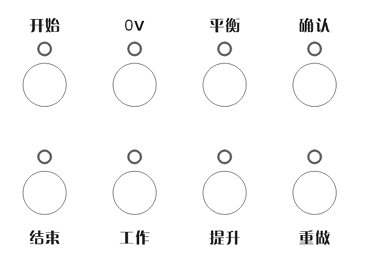
\includegraphics[width=0.6\textwidth]{figure6.png}
    \caption{仪器功能键示意图}
    \label{fig:instrument_keys}
\end{figure}

\paragraph{成像系统与界面操作}
喷入油雾后，在监视器上寻找大量运动的油滴像。若成像模糊，通过调焦旋钮进行调节直到清晰。若发生极板微孔堵塞，需断电后清理上极板。
实验界面会实时显示极板电压（范围 $0\text{--}999\text{ V}$）和经历时间（范围 $0\text{--}99.99\text{ s}$）。按“开始”键启动秒表，按“结束”键停止计时并自动记录数据。“0V”键用于使极板电压归零，使油滴在重力场中下落；“平衡”与“提升”键用于控制油滴的升降状态。

\paragraph{油滴的选择与控制练习}
实验成功的关键在于选择合适的油滴。应选取体积适中、成像清晰且带电荷量较少的油滴。建议选择平衡电压在 $150\text{--}400\text{ V}$ 之间、下落时间（距离 $2\text{ mm}$ 时）在 $20\text{ s}$ 左右的油滴。
在测量前，先调节电压使油滴停留在某一格线上观察其是否漂移，以确认力学平衡。练习通过切换“0V”和“平衡/提升”状态来控制油滴在特定格线区间内运动。

\paragraph{正式测量：平衡法}
在工作界面将状态切至“平衡”，选取油滴并调节电压使其在起始格线平衡。随后按“0V”使油滴自由下落，当油滴经过第一个标记线时按“开始”计，经过第二个标记线时按“结束”计。系统将自动记录该次电压与下落时间。之后按“提升”键将油滴提回起始位置上方，再次切回“平衡”状态使其稳定。
重复上述步骤完成 5 组数据记录。系统将根据采集的数据计算油滴电量 $Q$。为了验证电荷的量子化，建议测量多个不同油滴的电量，并寻找其最大公约数，或将测量值除以公认值 $e = 1.60 \times 10^{-19}\text{ C}$ 进行验证。

\begin{figure}[htbp]
    \centering
    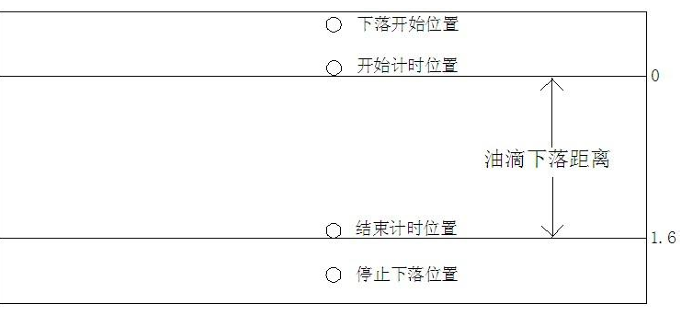
\includegraphics[width=0.5\textwidth]{figure7.png}
    \caption{平衡法/动态法测量区间示意图}
    \label{fig:measurement_diagram}
\end{figure}

\paragraph{正式测量：动态法}
动态法包含下落和提升两个阶段。第一步测量下落时间，操作方法与平衡法一致。第二步是在油滴落到低位后，通过增加极板电压使油滴上升，记录油滴向上经过标记区间的时间 $t_r$ 以及对应的提升电压 $U$。重复 5 次实验，利用动态法相关公式求得油滴电量 $Q$。

\paragraph{实验数据处理说明}
完成 5 组实验数据后，按“确认”键进行处理。监视器将显示油滴的平均电压、平均时间和所带电量。通过对比多个油滴的数据，可以验证电荷的不连续性，即所有电荷量都是基本电荷 $e$ 的整数倍。

\subsection{粘滞实验步骤}

\paragraph{实验准备与温度控制}
检查粘度测量仪和多功能温控实验系统的导线是否连接正确。设定实验所需的 PID 参数及实验温度，按启动键开始加热或制冷。本仪器的 PID 参数基于理论分析与大量实验得出，已达到最佳控制状态，通常无需调节。在初始加热阶段，PID 程序会自动调整温度略高于设定值（“过冲”现象），这是为了使蓖麻油能快速加热，属于正常功能设置。

\paragraph{测量小球直径}
使用千分尺或读数显微镜测量小球的直径 $d$。根据理论分析，当液体粘度及小球密度一定时，雷诺数 $\text{Re} \propto d^3$。在测量蓖麻油粘度时，建议采用直径 $1\text{--}2\text{ mm}$ 的小球，以忽略或仅考虑一级雷诺数修正。重复测量多次并将数据填入表 1。

\begin{table}[htbp]
\centering
\caption{小球的直径}
\begin{tabular}{lccccccccc}
\toprule
次数 & 1 & 2 & 3 & 4 & 5 & 6 & 7 & 8 & 平均值 \\
\midrule
$d$ ($10^{-3} \text{ m}$) & & & & & & & & & \\
\bottomrule
\end{tabular}
\end{table}

\paragraph{测定落体速度与计算粘度}
待温控仪达到设定温度后，需额外等待约 6 至 10 分钟。加热过程中，利用磁力棒在玻璃管外吸住管内的磁铁方块上下移动，通过搅拌液体加速热交换，确保样品管内待测液体的温度与显示温度完全一致。

实验相关参数如下：
\begin{itemize}
    \item 小球密度 $\rho = 7.8 \times 10^3 \text{ kg/m}^3$
    \item 液体密度 $\rho_0 = 0.95 \times 10^3 \text{ kg/m}^3$
    \item 玻璃管内径 $D = 2.6 \times 10^{-2} \text{ m}$
    \item 小球下落距离 $L = 0.2 \text{ m}$（上下刻度线垂直距离）
\end{itemize}

用镊子将干净的小球从漏斗中心轻轻放入液体，观察小球是否沿中心下落。若样品管倾斜，应调节其铅直状态。用停表测量小球落过距离 $L$ 所用的时间 $t$，计算其速度 $v_0$。根据修正后的斯托克斯公式计算粘度 $\eta$：
\begin{equation}
    \eta = \frac{(\rho - \rho_0)gd^2}{18v_0(1 + 2.4 d/D)}
\end{equation}

\paragraph{多温度点测定与数据记录}
根据实验要求选定多个温度点进行测量。如果时间紧张，可按教师要求在小组内分配测量任务。将测量结果填入表 2，并与提供的标准值进行比较，计算相对误差。

\begin{table}[htbp]
\centering
\caption{粘度的测定数据记录表}
\small
\begin{tabular}{cccccccccc}
\toprule
温度 & \multicolumn{6}{c}{时间 $t$ (s)} & 速度 & $\eta$ (Pa·s) & $*\eta$ (Pa·s) \\
\cmidrule(lr){2-7}
($^\circ$C) & 1 & 2 & 3 & 4 & 5 & 平均 & $v_0$ (m/s) & 测量值 & 标准值 \\
\midrule
25 & & & & & & & & & 0.621 \\
30 & & & & & & & & & 0.451 \\
35 & & & & & & & & & 0.312 \\
40 & & & & & & & & & 0.231 \\
45 & & & & & & & & & 0.172 \\
50 & & & & & & & & & 0.126 \\
55 & & & & & & & & & 0.098 \\
\bottomrule
\end{tabular}
\end{table}

\paragraph{实验收尾与绘图}
根据测量得到的 $\eta$ 值在坐标纸上作图，表明粘度随温度的变化关系。全部实验完成后，用磁铁棒将钢球和磁铁方块整体吸至管口，用镊子将钢球取出保存，并将磁铁方块放回蓖麻油中，盖好漏斗盖。


\section{实验数据与分析}
\subsection{密里根油滴实验的实验数据}
\begin{table}[htbp]
    \centering
    \caption{电压与时间测量数据记录表1}
    \begin{tabular}{cc}
        \toprule
        电压 / V & 时间 / s \\
        \midrule
        160 & 15.76 \\
        160 & 15.81 \\
        160 & 15.86 \\
        160 & 15.84 \\
        160 & 15.59 \\
        \midrule
        \multicolumn{2}{l}{计算结果：} \\
        平均电压 $V = 160 \text{ V}$ & 平均时间 $t = 15.83 \text{ s}$ \\
        \multicolumn{2}{l}{电荷量 $q = 8.9506 \times 10^{-19} \text{ C}$} \\
        \bottomrule
    \end{tabular}
\end{table}
\begin{table}[htbp]
    \centering
    \caption{电压与时间测量数据记录表 2}
    \begin{tabular}{cc}
        \toprule
        电压 / V & 时间 / s \\
        \midrule
        167 & 5.98 \\
        167 & 6.15 \\
        165 & 6.13 \\
        167 & 6.08 \\
        167 & 6.11 \\
        \midrule
        \multicolumn{2}{l}{计算结果：} \\
        平均电压 $V = 166 \text{ V}$ & 平均时间 $t = 6.09 \text{ s}$ \\
        \multicolumn{2}{l}{电荷量 $q = 3.7818 \times 10^{-18} \text{ C}$} \\
        \bottomrule
    \end{tabular}
\end{table}

\begin{table}[htbp]
    \centering
    \caption{电压与时间测量数据记录表 3}
    \begin{tabular}{cc}
        \toprule
        电压 / V & 时间 / s \\
        \midrule
        176 & 16.95 \\
        176 & 17.41 \\
        176 & 16.79 \\
        176 & 17.61 \\
        176 & 16.67 \\
        \midrule
        \multicolumn{2}{l}{计算结果：} \\
        平均电压 $V = 176 \text{ V}$ & 平均时间 $t = 17.08 \text{ s}$ \\
        \multicolumn{2}{l}{电荷量 $q = 7.2265 \times 10^{-19} \text{ C}$} \\
        \bottomrule
    \end{tabular}
\end{table}

\begin{table}[htbp]
    \centering
    \caption{电压与时间测量数据记录表4}
    \begin{tabular}{cc}
        \toprule
        电压 / V & 时间 / s \\
        \midrule
        214 & 13.48 \\
        214 & 12.96 \\
        214 & 13.19 \\
        214 & 13.36 \\
        212 & 13.01 \\
        \midrule
        \multicolumn{2}{l}{计算结果：} \\
        平均电压 $V = 213 \text{ V}$ & 平均时间 $t = 13.20 \text{ s}$ \\
        \multicolumn{2}{l}{电荷量 $q = 8.9229 \times 10^{-19} \text{ C}$} \\
        \bottomrule
    \end{tabular}
\end{table}

\begin{table}[htbp]
    \centering
    \caption{电压与时间测量数据记录表5}
    \begin{tabular}{cc}
        \toprule
        电压 / V & 时间 / s \\
        \midrule
        181 & 22.05 \\
        181 & 22.51 \\
        181 & 22.21 \\
        181 & 22.13 \\
        181 & 22.2  \\
        \midrule
        \multicolumn{2}{l}{计算结果：} \\
        平均电压 $V = 181 \text{ V}$ & 平均时间 $t = 22.22 \text{ s}$ \\
        \multicolumn{2}{l}{电荷量 $q = 4.6539 \times 10^{-19} \text{ C}$} \\
        \bottomrule
    \end{tabular}
\end{table}

\subsubsection{密立根油滴实验结果计算与分析}

根据上述 5 组测量数据，已知公认的基本电荷值 $e_{std} \approx 1.602 \times 10^{-19} \text{ C}$。

\subsubsection{基本电荷测量值的计算}
首先计算电荷量 $q$ 与 $e_{std}$ 的比值 $n' = q / e_{std}$，取最接近的整数 $n$ 作为油滴所带的基本电荷数。
然后由公式 $e_i = q_i / n_i$ 计算每次测量的基本电荷值。计算结果如下表所示：

\begin{table}[htbp]
    \centering
    \caption{基本电荷测量结果计算表}
    \begin{tabular}{ccccc}
        \toprule
        序号 & 总电荷量 $q$ / ($10^{-19} \text{ C}$) & $q/e_{std}$ & 电荷数 $n$ & 测量值 $e_i$ / ($10^{-19} \text{ C}$) \\
        \midrule
        1 & 8.9506 & 5.587 & 6 & 1.4918 \\
        2 & 37.8180 & 23.606 & 24 & 1.5758 \\
        3 & 7.2265 & 4.511 & 5 & 1.4453 \\
        4 & 8.9229 & 5.570 & 6 & 1.4872 \\
        5 & 4.6539 & 2.905 & 3 & 1.5513 \\
        \bottomrule
    \end{tabular}
\end{table}

\subsubsection{实验结果统计}
1. \textbf{平均值计算}

基本电荷的平均测量值为：
\[ \bar{e} = \frac{1}{5} \sum_{i=1}^{5} e_i = \frac{1.4918 + 1.5758 + 1.4453 + 1.4872 + 1.5513}{5} \times 10^{-19} = 1.5103 \times 10^{-19} \text{ C} \]

2. \textbf{不确定度分析}

根据贝塞尔公式，单次测量的标准偏差 $s$ 为：
\[ s = \sqrt{\frac{\sum_{i=1}^{5} (e_i - \bar{e})^2}{n-1}} = 0.0526 \times 10^{-19} \text{ C} \]

A 类标准不确定度 $u_A$：
\[ u_A = \frac{s}{\sqrt{5}} = \frac{0.0526}{2.236} \times 10^{-19} \approx 0.0235 \times 10^{-19} \text{ C} \]

相对不确定度 $u_r$：
\[ u_r = \frac{u_A}{\bar{e}} \times 100\% = \frac{0.0235}{1.5103} \times 100\% \approx 1.56\% \]

3. \textbf{最终结果表达}
\[ e = \bar{e} \pm u_A = (1.51 \pm 0.02) \times 10^{-19} \text{ C} \]

4. \textbf{误差分析}

与公认值 $e_{std} = 1.602 \times 10^{-19} \text{ C}$ 相比，相对误差 $E$ 为：
\[ E = \frac{|\bar{e} - e_{std}|}{e_{std}} \times 100\% = \frac{|1.5103 - 1.602|}{1.602} \times 100\% \approx 5.72\% \]

\textbf{分析讨论：}

本次实验测得的电子电荷平均值约为 $1.51 \times 10^{-19} \text{ C}$，与公认值的相对误差为 5.72\%。
从数据来看，测量值普遍偏小，且部分数据的电荷数 $n$ 并不接近整数（如第 1、3 组），这可能源于实验系统的系统误差。
可能的原因包括：实验环境温度变化导致油的密度和空气粘滞系数发生微小变化未被修正；显微镜读数或计时存在的偶然误差；以及计算公式中斯托克斯定律修正系数的近似性带来的误差。
尽管存在一定误差，但实验结果在数量级上正确，并大致验证了电荷的量子化性质。

\subsection{粘滞系数实验数据处理与结果}

本次实验中，使用的常数参数如下：
\begin{itemize}
    \item 重力加速度 $g = 9.793 \, \text{m/s}^2$
    \item 小球密度 $\rho = 7.8 \times 10^3 \, \text{kg/m}^3$
    \item 液体（蓖麻油）密度 $\rho_0 = 0.95 \times 10^3 \, \text{kg/m}^3$
    \item 玻璃管内径 $D = 2.6 \times 10^{-2} \, \text{m}$
    \item 小球下落距离 $L = 0.200 \, \text{m}$
    \item 小球直径 $d = (1.20 \pm 0.01) \times 10^{-3} \, \text{m}$
\end{itemize}

计算公式：
\[ v_0 = \frac{L}{t}, \quad \eta = \frac{(\rho - \rho_0)gd^2}{18v_0(1 + 2.4 d/D)} \]

代入已知数据可算得粘滞系数计算公式的系数：
\[ K = \frac{(\rho - \rho_0)gd^2}{18 L (1 + 2.4 d/D)} \approx 0.02416 \, \text{Pa}\cdot\text{s/s} \]
即 $\eta = K \cdot t$。

\begin{table}[htbp]
\centering
\caption{粘度的测定数据记录与结果表}
\label{tab:viscosity_result}
\resizebox{\textwidth}{!}{
\begin{tabular}{ccccccc}
\toprule
温度 ($^\circ$C) & 平均时间 $t$ (s) & 速度 $v_0$ (m/s) & 测量值 $\eta$ (Pa·s) & 标准值 $*\eta$ (Pa·s) & 相对误差 \\
\midrule
25 & 35.702 & 0.0056 & 0.8625 & 0.621 & 38.89\% \\
30 & 24.242 & 0.0083 & 0.5856 & 0.451 & 29.85\% \\
35 & 14.574 & 0.0137 & 0.3521 & 0.312 & 12.85\% \\
40 & 11.802 & 0.0170 & 0.2851 & 0.231 & 23.42\% \\
45 & 10.120 & 0.0198 & 0.2445 & 0.172 & 42.15\% \\
50 & 7.676 & 0.0261 & 0.1854 & 0.126 & 47.14\% \\
55 & 6.020 & 0.0332 & 0.1454 & 0.098 & 48.37\% \\
\bottomrule
\end{tabular}
}
\end{table}

\textbf{误差分析：}
实验结果显示，测量得到的粘滞系数普遍高于标准值，特别是在高温区和低温区相对误差较大。
这主要源于实际使用的小球直径（$1.20 \text{mm}$）可能与实验条件（如管壁效应修正系数的适用性或实际温度控制）存在一定偏差。
此外，液体密度变化和温度测量的准确性也是重要的误差来源。
\section{思考题解答}

\subsection{密立根油滴实验部分}

\begin{enumerate}
    \item \textbf{对实验结果造成影响的主要因素有哪些？} \\
    主要因素包括：空气粘滞系数受温度变化的影响；油滴在下落过程中因蒸发导致质量改变；实验过程中的布朗运动干扰；计时器的人为反应误差；极板电压的波动以及极板是否严格水平等。

    \item \textbf{若平行极板不水平，对测量量有何影响？} \\
    若极板不水平，电场力与重力方向不在同一直线上。这将导致油滴在运动过程中产生水平方向的漂移，使其容易离开视场。同时，电场力与重力的平衡条件被破坏，导致计算出的电荷量产生偏差。

    \item \textbf{如何选择合适的油滴进行测量？} \\
    应选择成像清晰、大小适中、带电量较少的油滴。太大的油滴重力大，下落和上升速度过快，计时误差大；太小的油滴受布朗运动影响剧烈，运动轨迹不稳定。通常建议选择平衡电压在 $150\text{--}400\text{ V}$，下落时间在 $20\text{ s}$ 左右的油滴。

    \item \textbf{实验上怎样做才能保证油滴做匀速运动？} \\
    在计时之前，应让油滴预先运动一段距离。对于受空气阻力的微小球体，阻力与速度成正比，它会在极短时间内达到受力平衡状态。只要避开起始加速阶段，并在稳定的气压环境下观察，即可近似认为其在测量区间内做匀速运动。

    \item \textbf{对油滴进行跟踪测量时，有时油滴逐渐变得模糊，为什么？} \\
    这主要是因为油滴在运动过程中偏离了显微镜的焦平面（景深较小）。此外，环境气流扰动或极板不水平导致油滴产生前后位移，也会使成像模糊。
\end{enumerate}

\subsection{落球法测定液体粘度部分}

\begin{enumerate}
    \item \textbf{斯托克斯定律的适用条件是什么？在实验中如何判断这些条件是否得到满足？如果小球下落速度过快，可能会对粘滞系数的测量结果产生什么影响？} \\
    适用条件为：液体是无限广阔的；小球是刚性的，且表面光滑；小球在液体中做匀速直线运动；雷诺数 $Re$ 极小（$Re < 0.1$）。实验中通过测量小球直径和速度计算 $Re$ 来判断。如果速度过快，$Re$ 增大，液体惯性力项不可忽略，会导致测得的阻力增大，从而使计算出的粘滞系数偏大。

    \item \textbf{实验中为什么要等待液体温度达到平衡后再开始测量？如果温度未稳定就进行实验，会对粘滞系数的测量带来怎样的误差？} \\
    液体的粘滞系数对温度极其敏感。等待温度平衡是为了确保测量的是该特定温度下的粘度。如果温度不稳定，液体内部可能存在温度梯度，导致粘度不均匀，甚至产生对流，从而使测量结果产生不可预测的随机误差或系统偏差。

    \item \textbf{在测量小球下落速度时，为什么要强调小球必须沿中心竖直下落？如果玻璃管倾斜，会对实验结果造成什么影响？} \\
    沿中心下落是为了减小壁效应对小球运动的影响（实验中已根据中心位置进行了修正）。如果玻璃管倾斜，小球会靠近管壁甚至摩擦管壁，使受到的阻力异常增大，同时下落路径变长，最终导致测得的粘滞系数偏大。
\end{enumerate}

\section{原始实验记录表和预习报告}
\begin{figure}
    \centering
    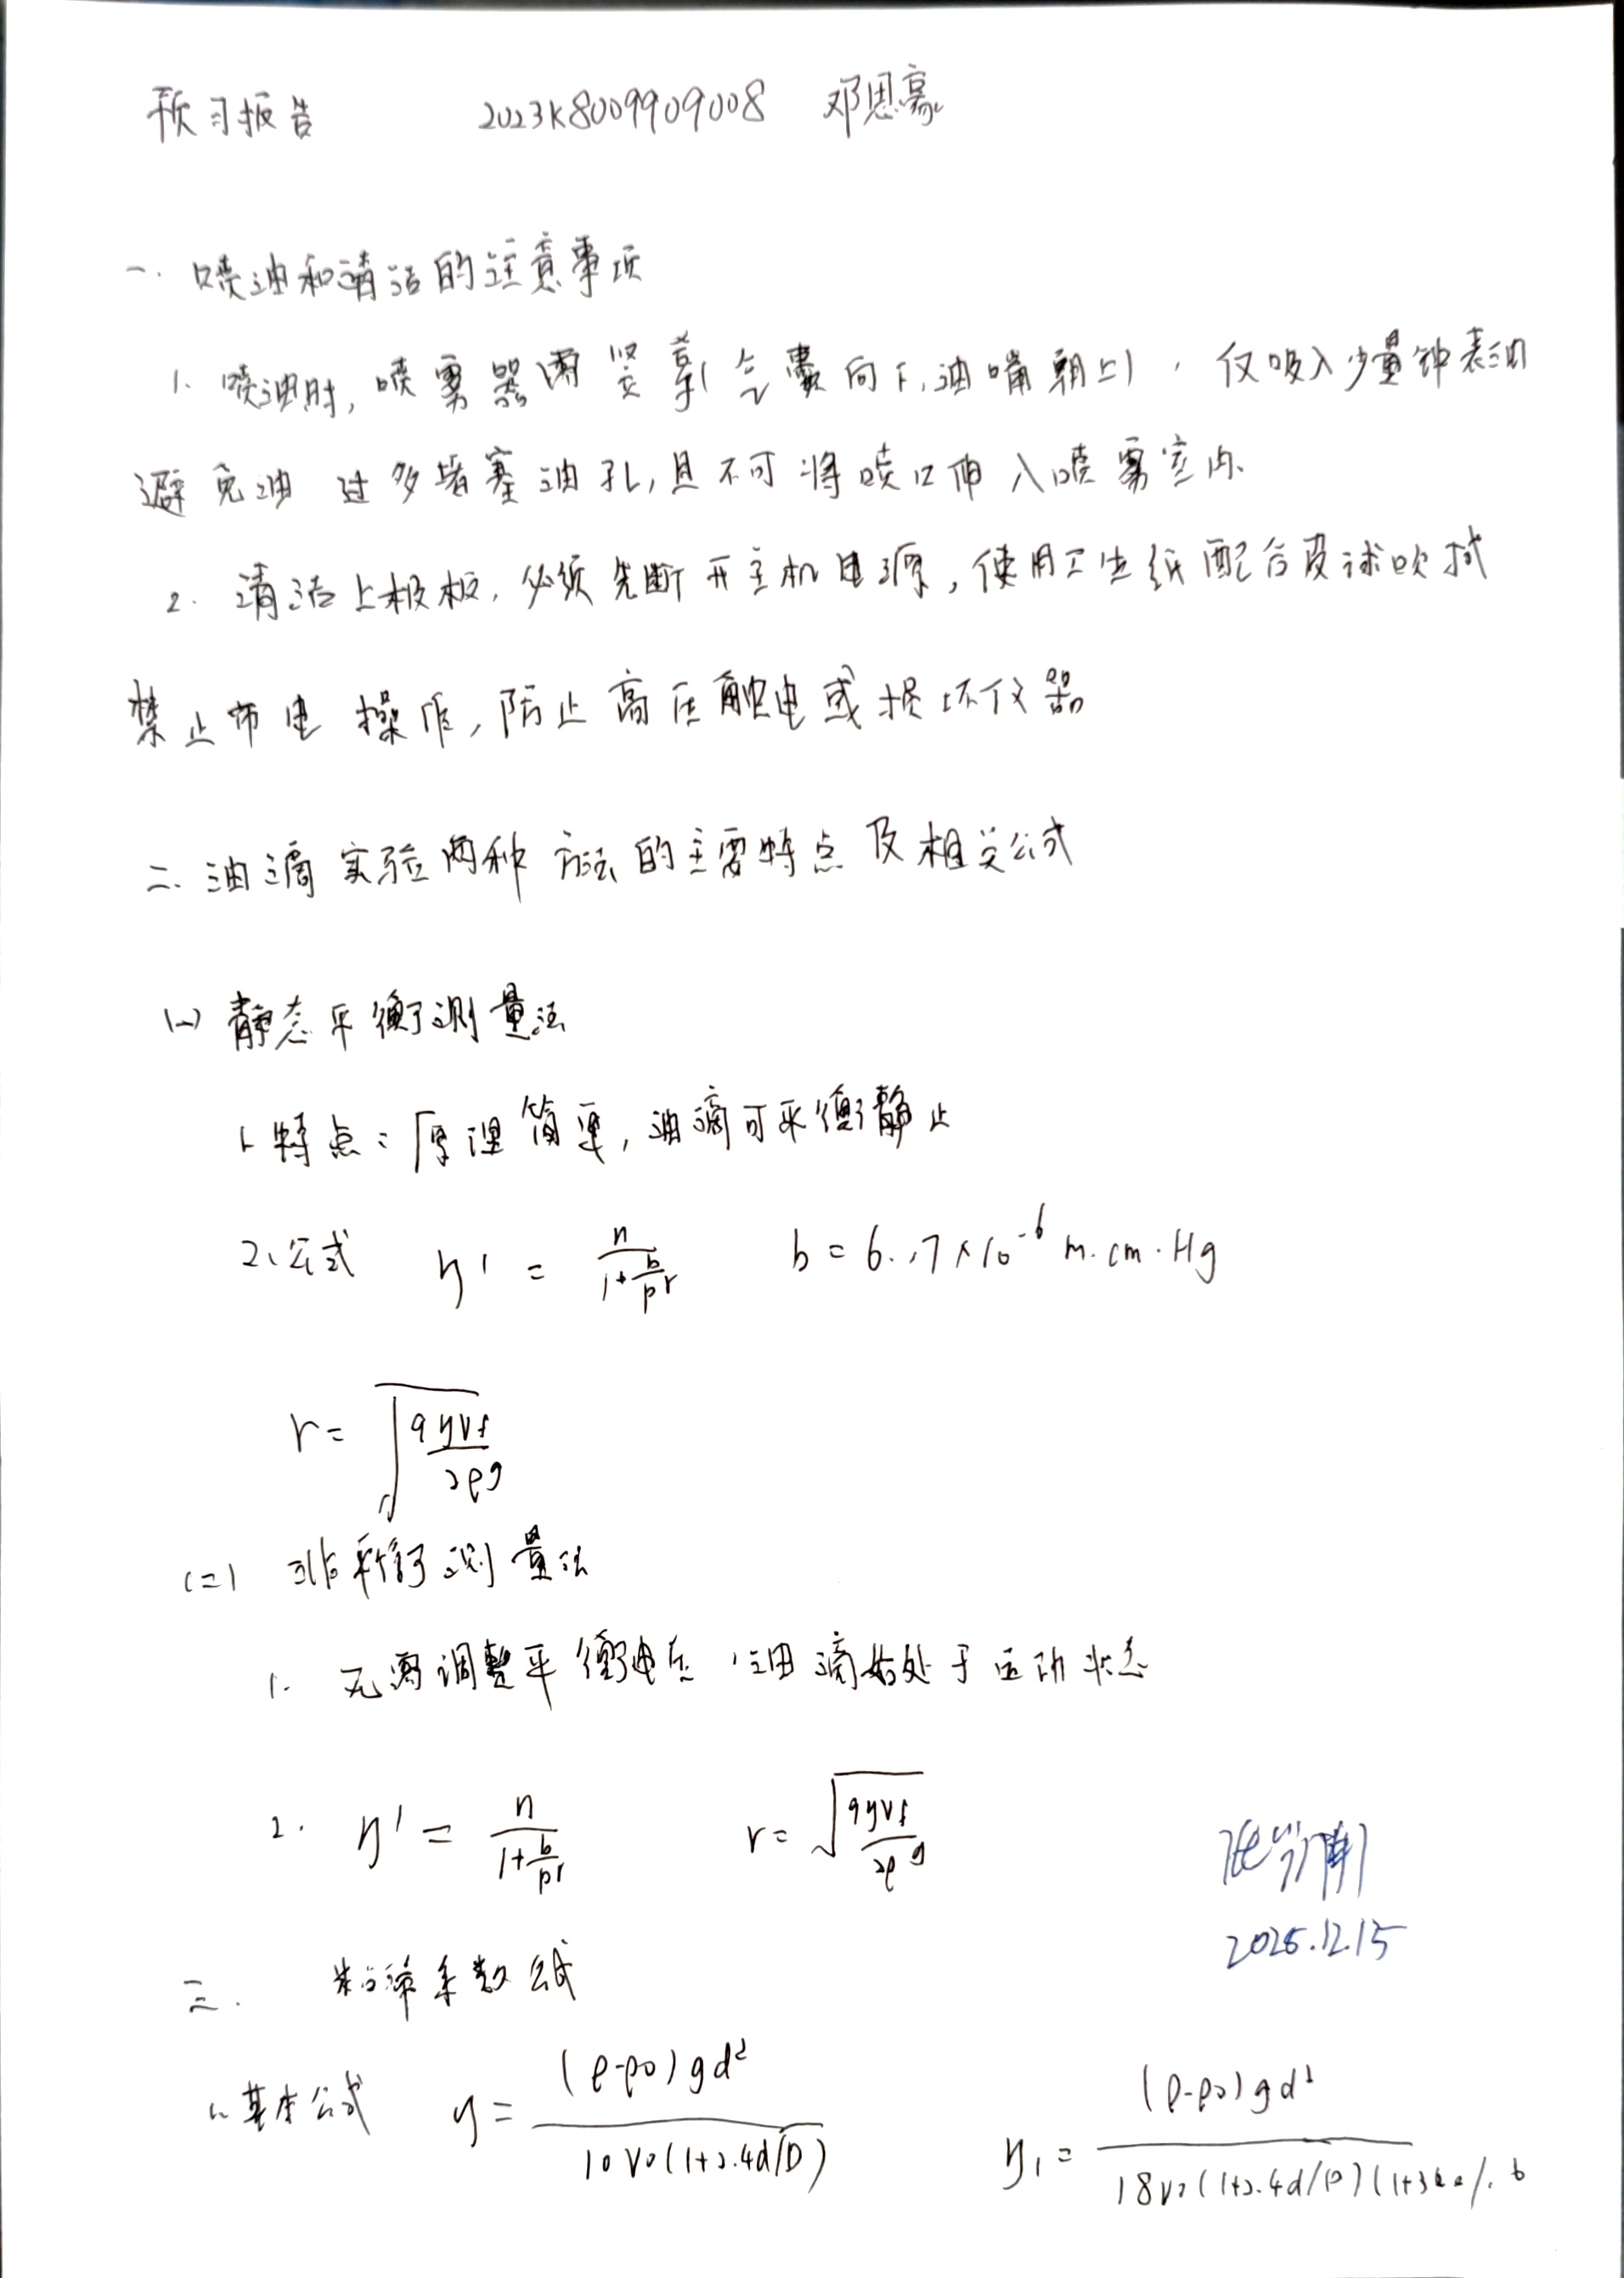
\includegraphics[width=0.8\textwidth]{IMG_20251215_135212.jpg}
    \caption{预习报告}
\end{figure}
\begin{figure}
    \centering
    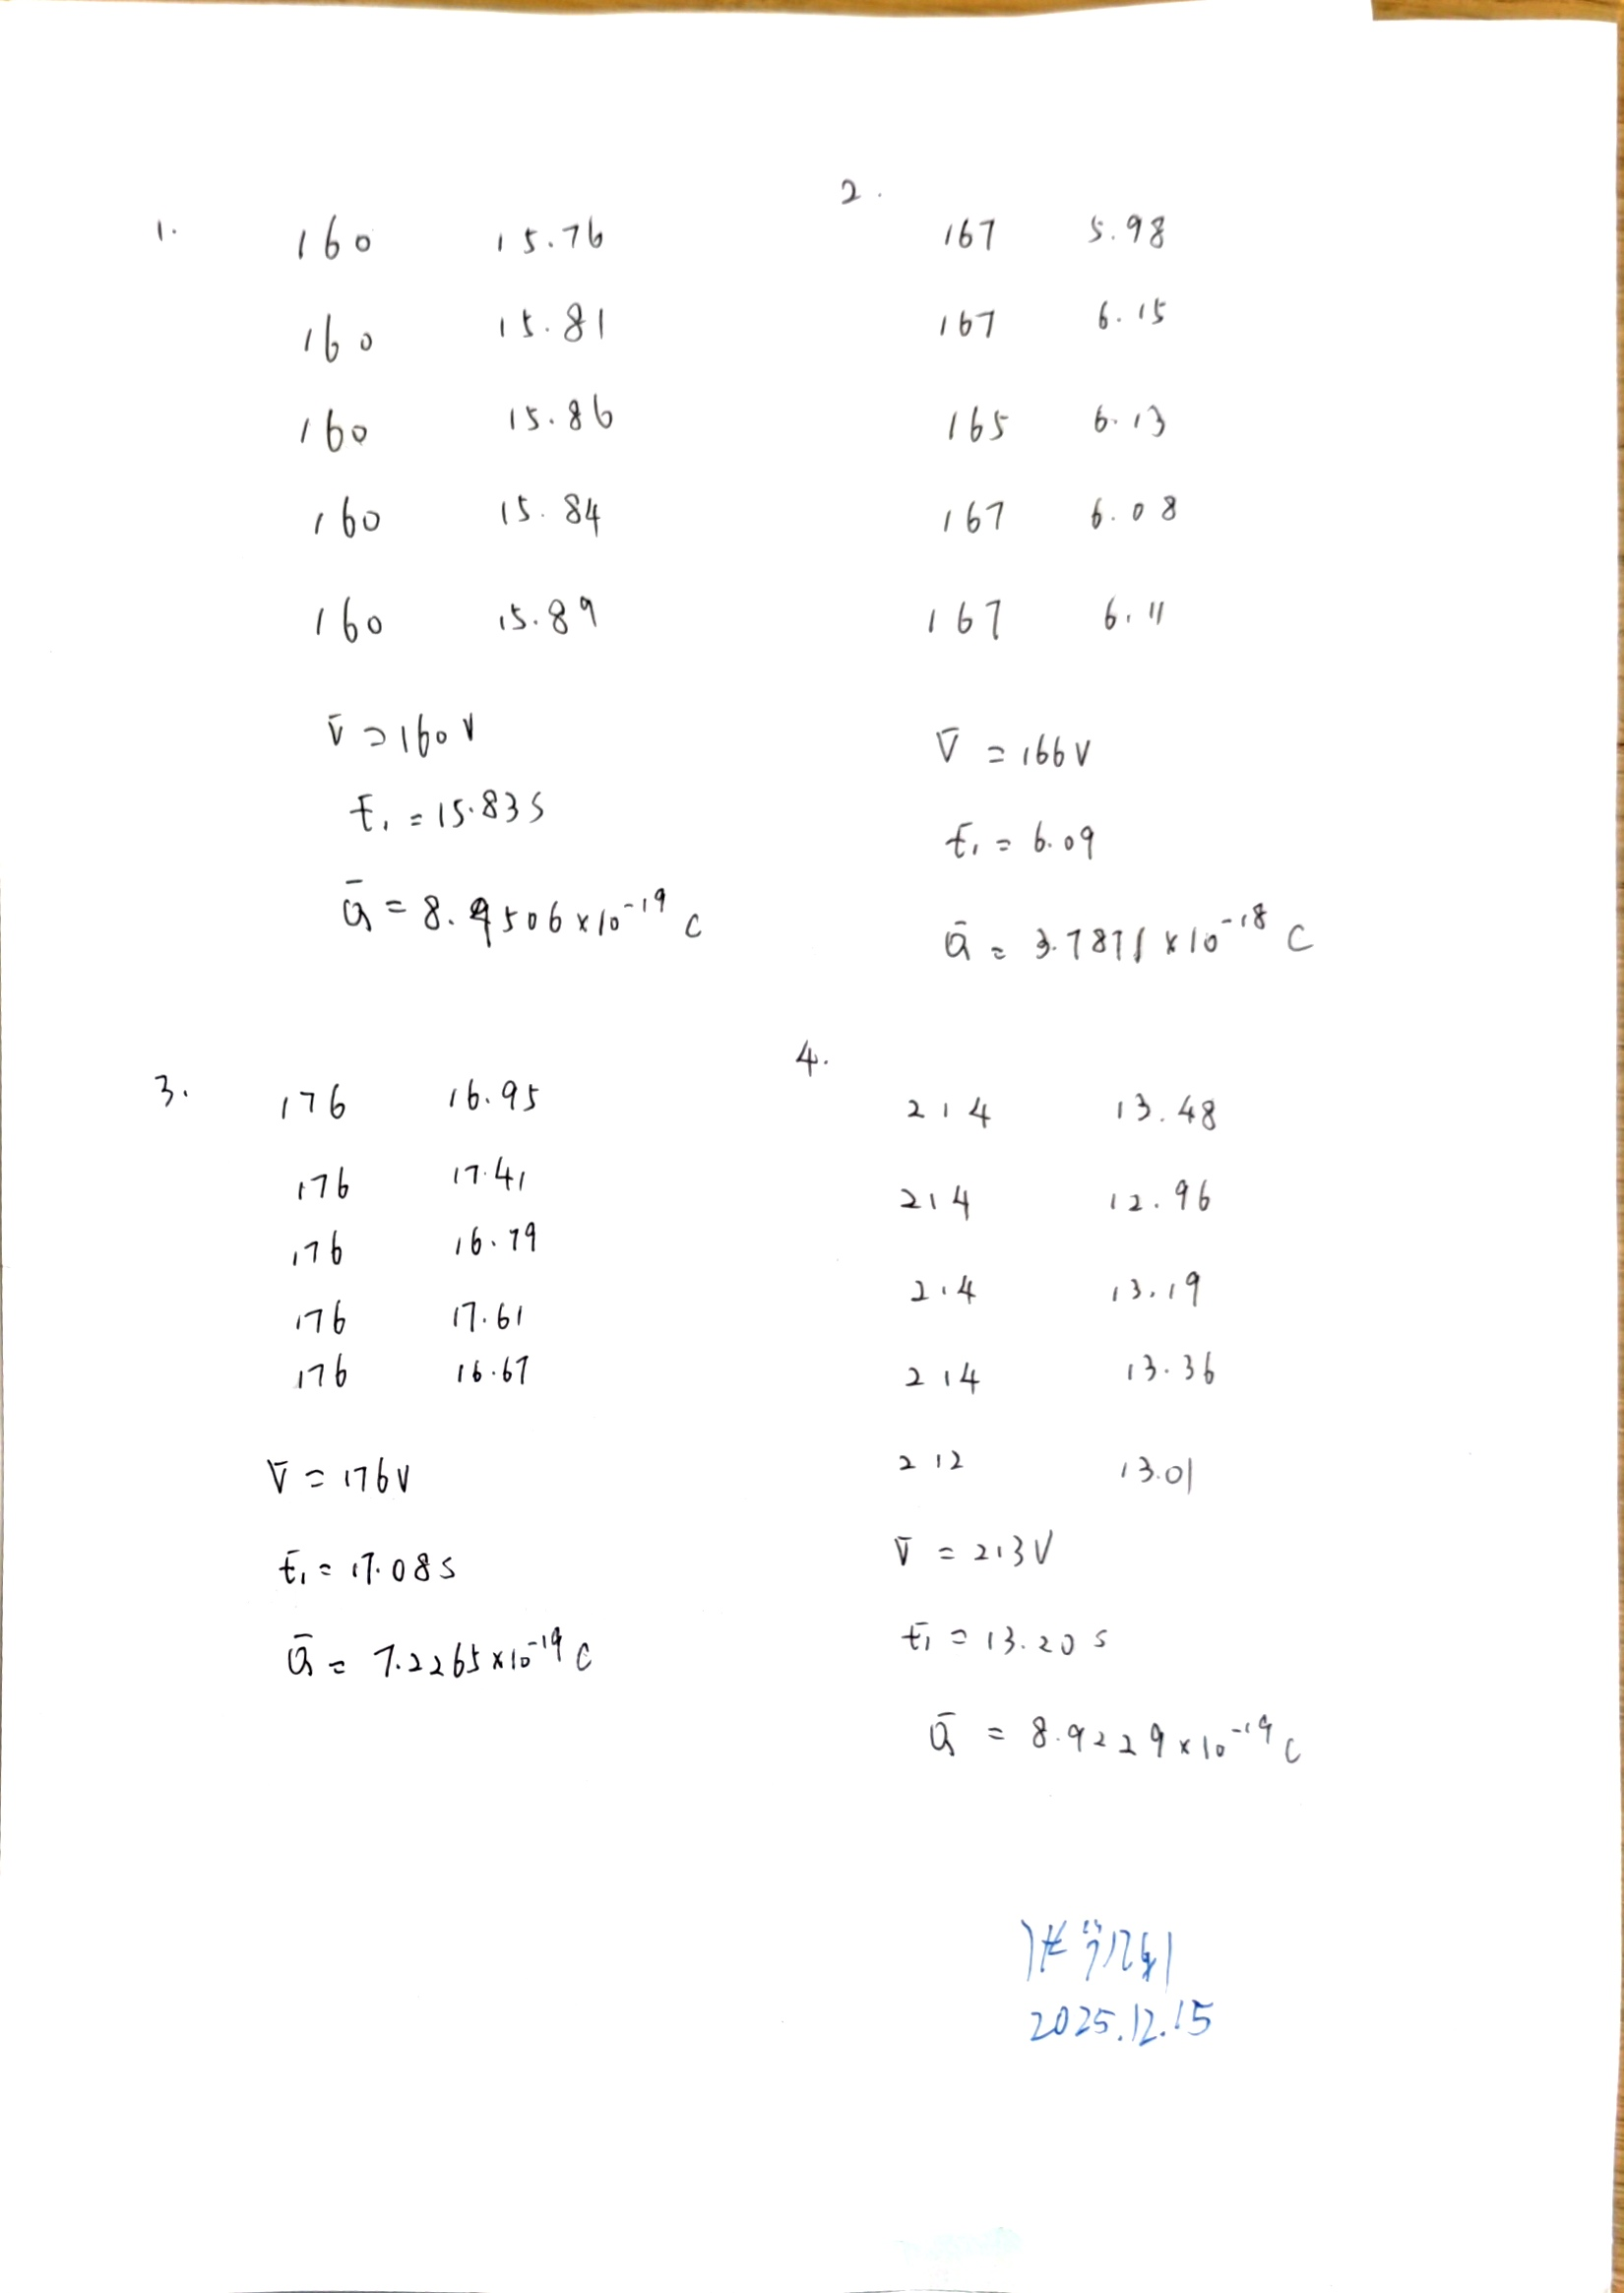
\includegraphics[width=0.8\textwidth]{IMG_20260213_162023.jpg}
    \caption{原始记录表1}
\end{figure}
\begin{figure}
    \centering
    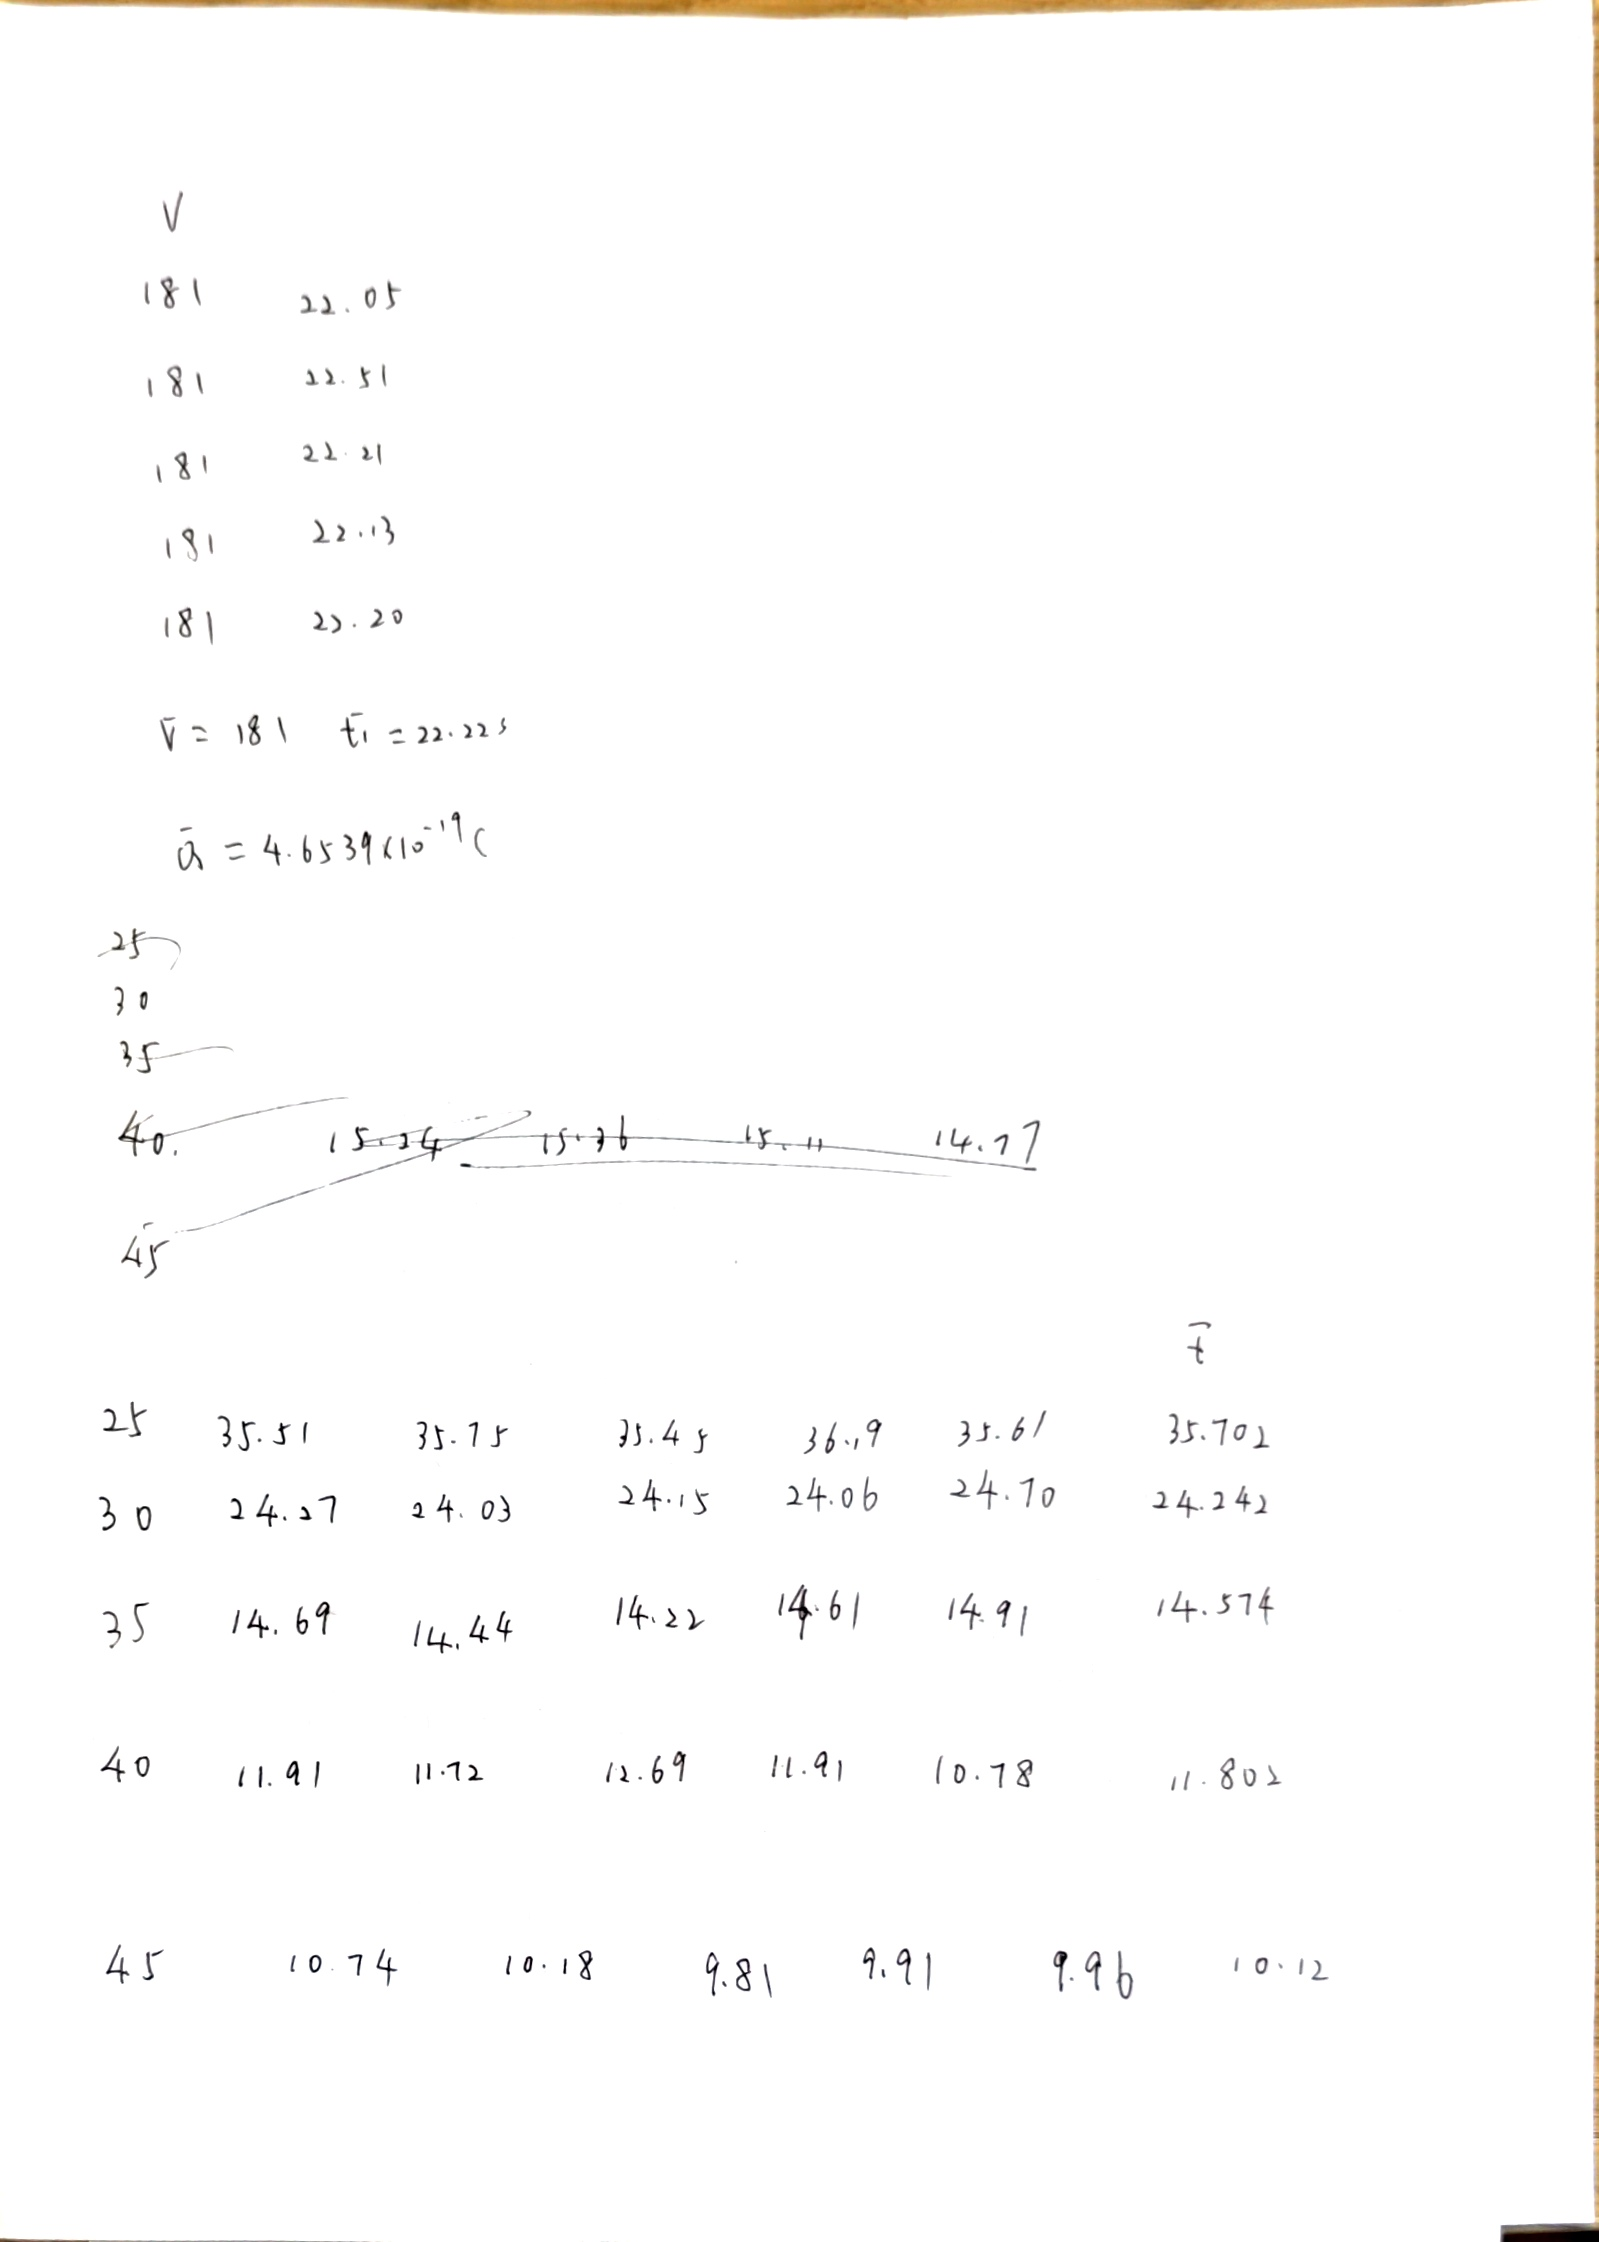
\includegraphics[width=0.8\textwidth]{IMG_20260213_162028.jpg}
    \caption{原始记录表2}
\end{figure}
\begin{figure}
    \centering
    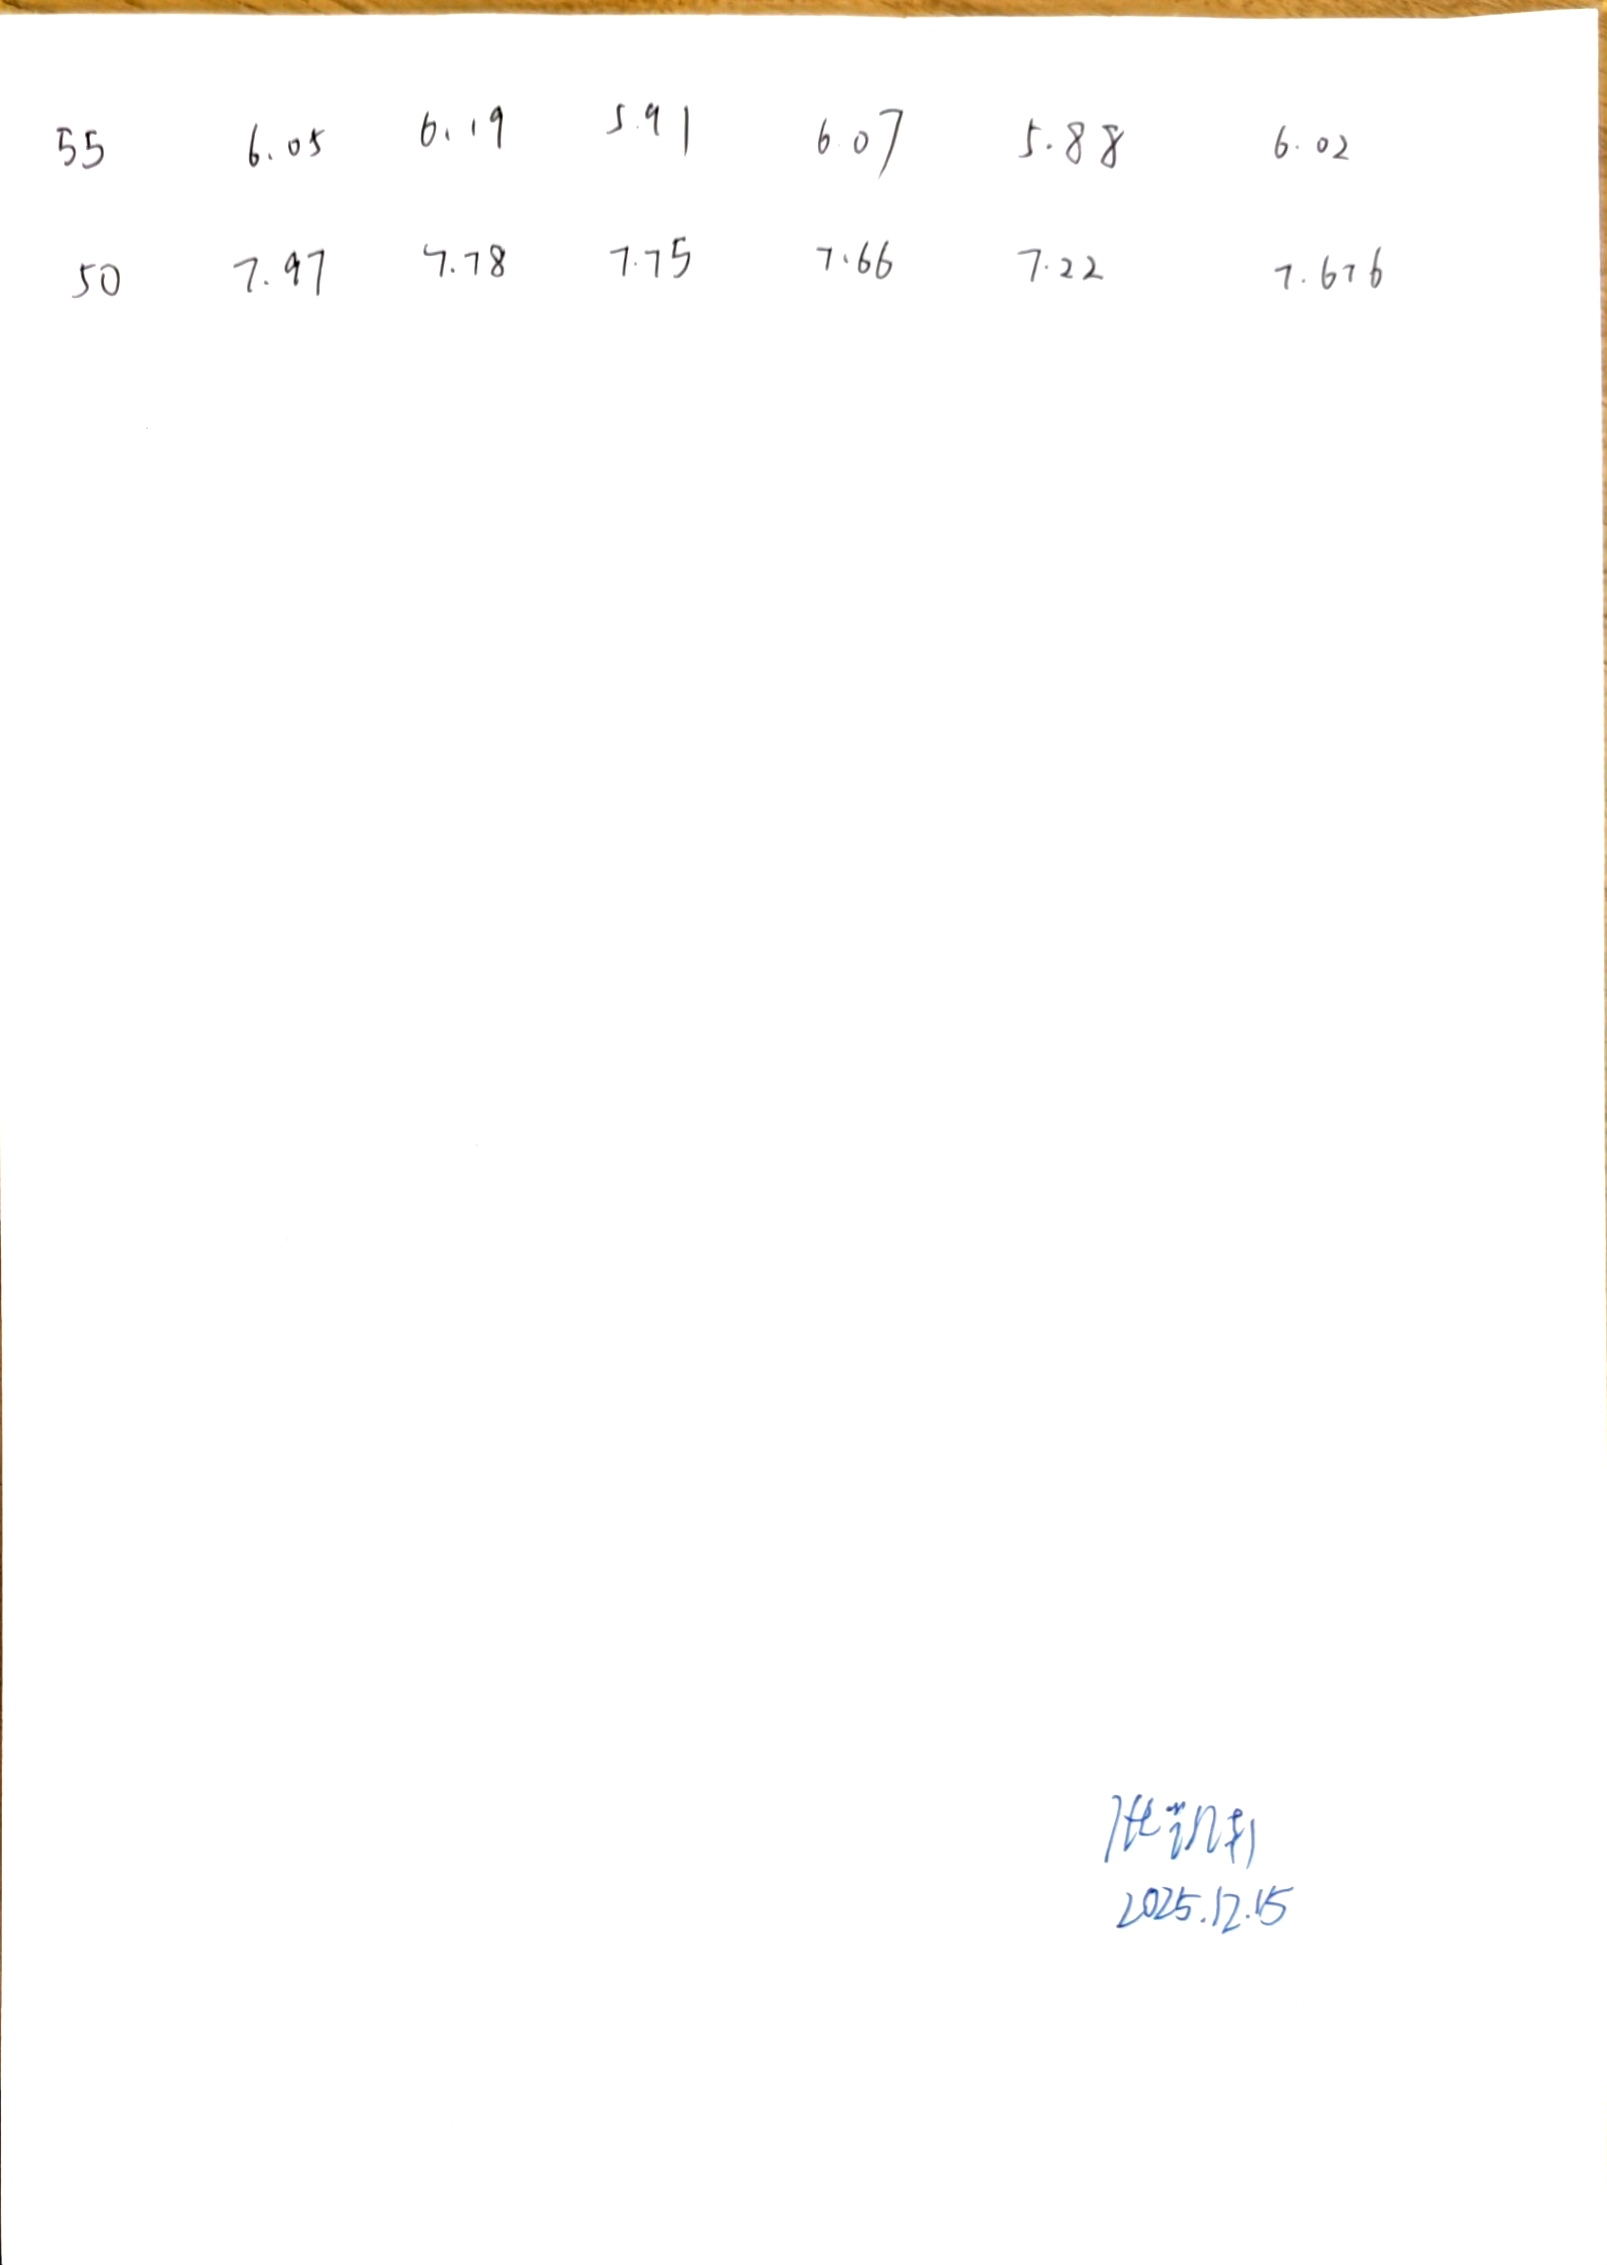
\includegraphics[width=0.8\textwidth]{IMG_20260213_162034.jpg}
    \caption{原始记录表3}
\end{figure}
\end{document}